\chapter{A ORGANIZAR}

\section{Cinemática Inversa}
Além do controle por velocidade do manipulador, utilizando a jacobiana inversa
para transformar comandos de velocidade desejada pelo usuário em velocidades das juntas, é possível controlar 
o braço robótico também por meio de inserção da posição e orientação desejadas, transformando
essas informações em valores das juntas por meio da cinemática inversa.

Inicialmente, assume-se que o usuário irá informar a posição e orientação da ferramenta em uso pelo
manipulador, ou do efetuador final, em relação ao sistema de coordenadas da estação. Esta relação entre 
sistema de coordenadas da ferramenta e estação pode ser transformado em uma relação 
entre os sistemas de coordenadas da última junta do manipulador em relação à primeira, da seguinte forma:

\begin{equation*}
    ^B_WT = ^B_S\!T\;^S_TT\;^W_TT^{-1}
\end{equation*}

A relação entre o punho, representado pelo \{$W$\}, do inglês \textit{wrist}, e a base \{B\},
é dada por:

\begin{equation*}
    ^B_WT = \; ^0_6T = 
    \begin{bmatrix}
        r_{11} & r_{12} & r_{13} & p_x \\
        r_{21} & r_{22} & r_{23} & p_y \\
        r_{31} & r_{32} & r_{33} & p_z \\
           0   &    0   &    0   &  1  \\    
    \end{bmatrix}
\end{equation*}

Para obter uma relação mais simples da geometria do robô é interessante ter uma relação 
entre a junta 5 a junta 1, portante, tanto a matriz acima quanto a matriz da equação \ref{eq:0T6}
serão multiplicadas por $^0_1T^{-1}$ e $^5_6T^{-1}$ na seguinte ordem:

\begin{equation*}
    ^1_5T = ^0_1\!T^{-1}\;^0_6T\;^5_6T^{-1}
\end{equation*}

Realizando esta transformação para a matriz que possui como parâmetros os ângulos das juntas
é obtido o seguinte resultado:

\begin{equation*}
    ^1_5T = 
    \begin{bmatrix}
        s_5c(\Theta) & c_5c(\Theta) & s(\Theta) & c(\Theta)a_5 + c(\theta_2+\theta_3)a_4 + c_2a_3 + a_2 \\
        c_5 & -s_5 & 0 & -(d_3+d_4) \\
        s_5s(\Theta) & c_5s(\Theta) & -c(\Theta) & s(\Theta)a_5+s(\theta_2+\theta_3)a_4 + s_2a_3 \\
           0   &    0   &    0   &  1  \\    
    \end{bmatrix}
\end{equation*}

onde,

\begin{equation*}
    \Theta = \theta_2+\theta_3+\theta_4
\end{equation*}

Agora, para a matriz $^0_6T$ com base nos parâmetros desejados, o obtido é:

\begin{equation*}
    ^1_5T = 
    \begin{bmatrix}
         c_1(r_{11}c_6-r_{12}s_6) &  c_1r_{13}+s_1r_{23} & -c_1(r_{11}s_6+r_{12}c_6) &  c_1(p_x-r_{13}d_6) \\
        +s_1(r_{21}c_6-r_{22}s_6) &                      & -s_1(r_{21}s_6+r_{22}c_6) & +s_1(p_y-r_{23}d_6) \\
        & & & & \\
        -s_1(r_{11}c_6-r_{12}s_6) & -s_1r_{13}+c_1r_{23} &  s_1(r_{11}s_6+r_{12}c_6) & -s_1(p_x-r_{13}d_6) \\
        +c_1(r_{21}c_6-r_{22}s_6) &                      & -c_1(r_{21}s_6+r_{22}c_6) & +c_1(p_y-r_{23}d_6) \\
        & & & & \\        
             r_{31}c_6-r_{32}s_6  &         r_{33}       &     -r_{31}s_6-r_{32}c_6  &      p_z-r_{33}d_6  \\
        & & & & \\
                    0             &            0         &              0            &           1         \\    
    \end{bmatrix}
\end{equation*}

Os termos $p_x-r_{13}d_6$ e $p_y-r_{23}d_6$ equivalem, respectivamente, às posições x e y da quinta junta no sistema 
de coordenadas da primeira junta, assim, alternando esses termos para suas respectivas coordenadas polares,
obtém-se:

\begin{align*}
    p_x - r_{13}d_6 &= \; ^1_5\rho_x = \; ^1_5\rho \cdot cos ^1_5\phi \\
    p_y - r_{23}d_6 &= \; ^1_5\rho_y = \; ^1_5\rho \cdot sen ^1_5\phi \\
\end{align*}

Substituindo os valores mais a direita no termo (2, 4) da matriz e igualando ao termo (2, 4) da matriz em função
das variáveis das juntas, chega-se à seguinte relação:

\begin{equation*}
    -s_1 \cdot ^1_5\rho \cdot cos ^1_5\phi + c_1 \cdot ^1_5\rho \cdot sen ^1_5\phi = - (d_3 + d_4)
\end{equation*}

, assim:

\begin{equation*}
    sen(\theta_1 - ^1_5\phi) = \frac{d_3+d_4}{^1_5\rho}
\end{equation*}

Utilizando a identidade trigonométrica fundamental, obtém-se também:

\begin{align*}
    cos(\theta_1 - ^1_5\phi) &= \pm \sqrt{1 - \frac{(d_3+d_4)^2}{^1_5\rho^2} } \\
                             &= \pm \frac{\sqrt{^1_5\rho_x^2 + ^1_5\rho_y^2 - (d_3+d_4)^2}}{^1_5\rho}  \\
\end{align*}

Essas duas equações levam ao seguinte resultado para o valor de $\theta_1$:

\begin{align*}
    \theta_1 &= ^1_5\phi + atan2\left(\frac{d_3+d_4}{^1_5\rho}, \frac{\sqrt{^1_5\rho_x^2 + ^1_5\rho_y^2 - (d_3+d_4)^2}}{^1_5\rho}\right) \\
             &= atan2(^1_5\rho_y, ^1_5\rho_x) + atan2\left(d_3+d_4,\sqrt{^1_5\rho_x^2 + ^1_5\rho_y^2 - (d_3+d_4)^2}\right) \\
\end{align*}

\section{others}

\label{A arrumar}
O que está descrito aqui será reescrito e reposicionado melhor no relatório final

% Resumo opcional. Comentar se não usar.
%\resumodocapitulo{Resumo opcional}

\section{Metodologias de projeto}
\label{sec:Fundamentos-Metodologias}

Durante o desenvolvimento de um processo/projeto, são empregadas diferentes ferramentas, abordagens e metodologias para implementar uma gestão da qualidade
deste. A maioria dessas técnicas de gestão são utilizadas em todo o mundo e são simples de entender, no entanto, algumas são mais complexas e demandam um 
maior esforço para serem incluídas no ciclo de vida do processo. É de extrema importância que uma metodologia seja devidamente escolhida e aplicada, 
sendo que o sucesso da sua implementação depende do entendimento e conhecimento acerca desta \cite{sokovic2010quality}.

Vários modelos de metodologias de gestão já foram criadas, com uma gama de aplicações, tanto para o desenvolvimento de \textit{softwares} quanto para o 
desenvolvimento de \textit{hardwares}, como o modelo cascata, espiral, modelo V e ágil. O modelo em cascata é o mais antigo de todos e o mais conhecido,
consistindo de uma sequência de estágios ligados diretamente, onde uma etapa do processo depende da etapa passada. Já o modelo em V demonstra a relação
entre cada fase do ciclo de desenvolvimento e a sua etapa de teste associada. A metodologia ágil surgiu com foco no desenvolvimento de projetos de 
\textit{software}, sendo baseada em iterações e incrementações contínuas, com requisições e soluções evoluindo através da colaboração das equipes
de desenvolvimento \cite{balaji2012waterfall}.

Outros métodos de gestão de qualidade criados propõem uma organização de trabalho mais cíclica, como no caso do ciclo PDCA, ou ciclo de Deming, onde são propostas 4 etapas
que caracterizam o nome desse método: Planejar (\textit{\textbf{P}lan}) - Fazer (\textit{\textbf{D}o}) - Checar (\textit\textbf{C}heck) - Agir (\textit{\textbf{A}ct}).
Este ciclo é considerado como um conceito de melhoria contínua, onde a cada repetição o processo apresenta melhorias em relação ao seu estado original. A metodologia
\textit{Six Sigma} também se baseia em uma melhoria contínua e cíclica do processo. Sendo vista fundamentalmente como uma metodologia para melhoria de processos
já existentes, uma variação do seu ciclo básico foi proposta sob o nome de Projeto para Seis Sigma (DFSS - \textit{Design For Six Sigma}), onde o ciclo de 
trabalho frequentemente é dividido em 5 etapas: Definir (\textit{\textbf{D}efine}) - Medir (\textit{\textbf{M}easure}) - Analisar (\textit{\textbf{A}nalyse}) -
Projetar (\textit{\textbf{D}esign}) - Verificar (\textit{\textbf{V}erify}), sendo este ciclo comumente referido como DMADV \cite{sokovic2010quality}.

\subsection{Cascata}
Como dito anteriormente, o modelo por cascata é um modelo de desenvolvimento sequencial, dada esta natureza, muitas vezes é empregado naturalmente. Neste método
cada passo depende da evolução do passo anterior, sem sobreposição temporal, portanto, é importante que as especificações do projeto sejam bem claras no início
do desenvolvimento, pois estas serão carregadas em todos os passos, assim como ilustrado na figura \ref{fig:Meth-Waterfall}. Dentre os pontos positivos deste 
método estão a alocação temporal específica para cada etapa, facilidade de implementação e a baixa quantidade de ferramentas necessárias para a implementação deste método com sucesso.

No entanto, este método apresenta alguns pontos ruins, como no caso em que há uma mudança nas especificações, esta não estaria prevista no processo de 
desenvolvimento, podendo chegar a não ser implementada. A sequencialidade do método também limita a adequação das etapas a erros, onde um erro pode ocasionar 
o atraso de todas as entregas subsequentes, resultando em um sistema mal estruturado \cite{balaji2012waterfall}. 

\begin{figure}[h]
\caption{Exemplo de fluxo de trabalho por método de cascata}    
\begin{centering}
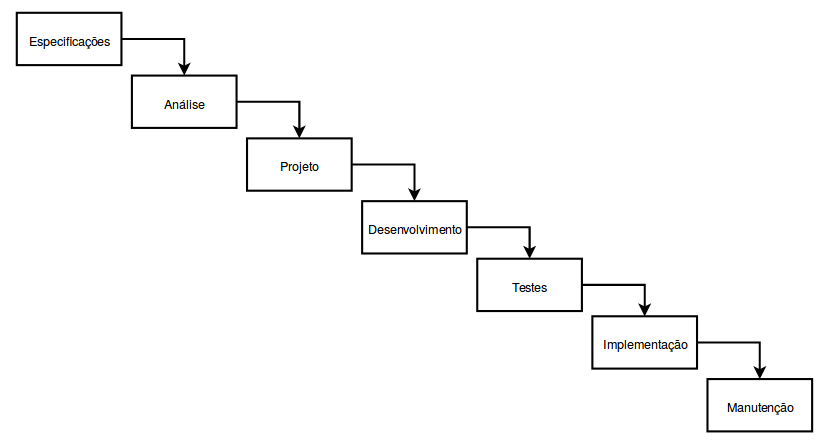
\includegraphics[width=1\columnwidth]{images/meth/Meth-Waterfall.png}
\par\end{centering}

\label{fig:Meth-Waterfall}

\end{figure}

A figura \ref{fig:Meth-Waterfall} exemplifica como a saída de uma etapa é a entrada da seguinte, assim como em uma cascata, evidenciando o nome do método de gestão.

% Falar do Modelo V?

\subsection{Ágil}
Desenvolvido primordialmente para a produção de \textit{softwares}, o manifesto ágil contém vários principios que ditam como deve ser o desenvolvimento de um 
produto, estes princípios prezam pela entrega contínua de código funcional, satisfação do cliente em mente, motivação da equipe e incrementações contínuas 
ao produto \cite{beck2001manifesto}. Diferentes técnicas e ferramentas são ligadas à metodologia ágil, como SCRUM, Desenvolvimento Adaptativo de \textit{Software} - DAS e Programação 
Extrema - XP, cada variação com práticas e terminologias próprias, prioridades diferentes e situações diferentes de aplicação \cite{kaisti2013agile}. 

O desenvolvimento de produtos com esta metodologia em mente aceita modificações nas especificações, até mesmo em estados tardios, sendo que um dos valores 
dispostos no manifesto ágil \cite{beck2001manifesto} é descrito como ``Responder a mudanças ao invés de seguir um plano'', tornando este método indicado em casos
onde as especificações não estão bem definidas no início. Para a aplicação de métodos ágeis no projeto de sistemas embarcados, incluindo \textit{hardware}, se 
fazem necessárias algumas adaptações, pois estas áreas de trabalho apresentam maiores restrições, como no caso de testes. No entanto, o uso diversas 
ferramentas e práticas aderentes a esta metodologia de gestão pode garantir um sucesso em diferentes situações durante as etapas de desenvolvimento \cite{kaisti2013agile}.

% Ilustrar o ágil?

% Falar do PDCA?

\subsection{Projeto para Seis Sigma}
Baseada na metodologia de melhoria de processos \textit{Six Sigma}, esta variação foi desenvolvida com foco em novos processos e produtos, com o objetivo principal
de ``Projetar correto na primeira vez'' \cite{yang2003design}. O conceito de sigma ($\sigma$) tem origem no ramo da estatística, referenciando o desvio padrão
de alguma medida, este conceito fundamenta a metodologia em questão, que busca limitar os resultados das medidas do processo/produto em um intervalo de seis 
vezes o seu desvio padrão, $\pm6\sigma$, indicando uma taxa de 99,9997$\%$ de acerto \cite{pande2001six}.

O Projeto para Seis Sigma é aplicável para a quase todos os tipos de desenvolvimento de projeto, mesmo que este necessite de uma grande variedade de ramos de 
engenharia diferentes. DFSS pode ser aplicado por meio de um ciclo de 5 estágios denominado DMADV, como explicado na seção \ref{sec:Fundamentos-Metodologias}.
O primeiro estágio consiste em contextualizar o produto e o que este se propõe a resolver, definindo seus objetivos primários. Durante o segundo estágio, 
o de medição, serão identificados parâmetros críticos e métricas que representam melhor o produto, estes dois estágios iniciais geram as especificações 
do produto final. Durante o terceiro estágio, serão analisadas alternativas de projeto e escolhida aquela mais proeminente. A próxima etapa consiste no desenvolvimento
em si, concretizando o produto através de protótipos e otimização. O último estágio do método realiza a verificação e adequação dos resultados finais ao que foi
proposto inicialmente e às medições de desempenho adotadas \cite{maass2009applying}.

\begin{figure}[h]
\caption{Ciclo DMADV para aplicação de DFSS}    
\begin{centering}
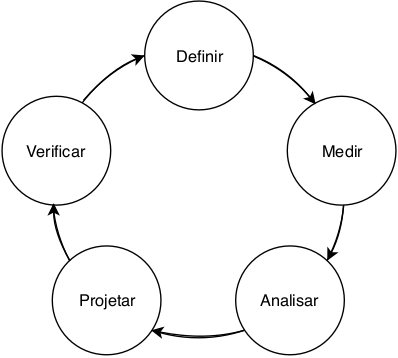
\includegraphics[width=0.5\columnwidth]{images/meth/DMADV.png}
\par\end{centering}

\label{fig:DMADV}
\end{figure}

A figura \ref{fig:DMADV} ilustra o ciclo de trabalho através desta metodologia. Por permitir uma maior flexibilidade na geração das especificações do projeto e
por não requerer uma extrema adaptação do método para produtos de \textit{hardware} e \textit{firmware}, este ciclo será o adotado ao longo do desenvolvimento 
deste projeto. 

Uma visão macro do ciclo empregado ao longo do desenvolvimento deste projeto, com base na metodologia escolhida, é detalhada como:

\begin{enumerate}
    \item Definição dos objetivos gerais do robô;
    \item Definição de requisitos técnicos buscados, como \textit{payload}, velocidade de atuação, precisão de posicionamento e capacidade de repetição de tarefas;
    \item Análise e comparação dos diversos tipos de atuadores, sensores, circuitos acionadores, processadores e controladores que podem ser empregados;
    \item Seleção de elementos com base na etapa passada e projeto das conexões entre estes;
    \item Verificação da adequação do sistema final proposto aos objetivos iniciais, otimização com base em diferenças observadas pela realimentação dessas em um novo ciclo de trabalho.
\end{enumerate}

A etapa de análise conta com o estudo de uma diversa gama de elementos para diferentes fins, para facilitar essa análise está será dividida em ciclos menores de 
trabalho paralelos para o projeto de atuadores e sensores, e em seguida, ciclos para o projeto dos circuitos de acionamento, processamento e controle, da seguinte
maneira:

\begin{enumerate}
    \item \begin{enumerate}
        \item Representação dos objetivos gerais em função dos atuadores e sensores;
        \item Levantamento de requisitos de torque, velocidade, precisão, custo e afins para atuadores e requisitos de precisão, disponibilidade, custo e afins para sensores;
        \item Análise em paralelo de sensores e atuadores que cumprem os respectivos requisitos;
        \item Seleção de elementos com base na análise;
        \item Verificação do cumprimento dos requisitos e otimização, início de novo ciclo para correção de parâmetros.
    \end{enumerate}
    \item \begin{enumerate}
        \item Levantamento de objetivos gerais para circuitos de acionamento;
        \item Geração de requisitos elétricos com base nos atuadores selecionados;
        \item Análise de topologias e elementos de potência para acionamento;
        \item Seleção;
        \item Testes e verificação de corretude do projeto de acionamento para os atuadores propostos.
    \end{enumerate}
    \item \begin{enumerate}
        \item Levantamento de objetivos gerais para circuitos de processamento e controle;
        \item Geração de requisitos de elementos condicionadores e processadores com base nos resultados de etapas passadas;
        \item Análise de possíveis soluções;
        \item Seleção;
        \item Verificação da comunicação entre todos os sistemas.        
    \end{enumerate}
\end{enumerate}

Em cada uma das etapas de verificação é possível que seja necessário uma revisão do que foi proposto na etapa anterior, dando continuidade aos ciclos até que todo
o sistema como um todo seja identificado como uma boa solução no macro ciclo de trabalho.

% Eplicar porque essa vai ser a melhor

\section{Motores}
Iniciando a seleção pelas juntas 5 e 6, que demandam um torque mais 
reduzido em comparação a outras juntas e realizam movimentos relativos ao
punho do manipulador, seria interessante empregar atuadores pequenos 
fisicamente mas que consigam fornecer a potência requerida pelo sistema, 
mantendo o efetuador final simples e sem muitas restrições mecânicas. 
No quesito de potência elétrica consumida, é ideal a escolha de atuadores 
eficientes que não resultem em gastos indesejados e evitáveis. Como o 
acionamento de motores de passo demanda sempre a corrente especificada, 
independente da carga, os motores de rotação contínua seriam uma melhor 
opção. Entretanto, para economizar potência na utilização de motores de 
passo, é possível desligar o seu acionamento quando este não estiver em 
uso, evitando perda por efeito Joule nas suas bobinas. 

Motores DC de rotação contínua apresentam também uma relação potência/peso 
frequentemente melhor frente aos motores de passo, garantindo mais um 
ponto positivo na escolha deste tipo de componentes. 
Ambos os tipos de atuadores em questão apresentam métodos de acoplamentos 
simples. Em relação ao acionamento e preço os motores de passo e motores 
com escova são as melhores opções, já em relação à durabilidade, os 
motores DC sem escovas, incluindo os motores de passo, apresentam uma 
vantagem frente aos aos motores DC escovados. Por fim, os motores de passo 
apresentam um bom comportamento mesmo em malha aberta, já outros tipos de 
motores DC requerem um maior processamento e componentes extras de 
sensoriamento e transmissão para obter resultados semelhantes, tanto em 
torque quanto precisão. 

Utilizando os parâmetros dispostos na seção de análise e pesos atribuídos 
a estes parâmetros, é possível simplificar a escolha dos atuadores para 
estas duas juntas em uma matriz de decisão, onde são atribuidas notas de 
1 a 5 para cada atuador, com base no cenário analisado, onde 5 indica uma 
ótima adequação. 
A matriz de decisão está representada na forma da tabela \ref{tab:SelAtuadores56}.

\begin{table}[h]
\begin{centering}    
    
\begin{tabular}{|c|c|c|c|c|}
    \hline
     & & Motor de passo & Motor DC com escovas & Motor DC sem escovas \tabularnewline
    \hline
    Parâmetro & Peso & & & \tabularnewline 
    \hline
    \hline
    Potência consumida & 3 & 2 & 3 & 4 \tabularnewline
    \hline
    Precisão & 3 & 4 & 2 & 2 \tabularnewline
    \hline
    Massa & 2 & 1 & 3 & 4 \tabularnewline
    \hline
    Inserção & 1 & 4 & 4 & 4 \tabularnewline
    \hline    
    Acionamento & 2 & 3 & 4 & 1 \tabularnewline
    \hline
    Custo & 4 & 3 & 3 & 1 \tabularnewline
    \hline
    Durabilidade & 4 & 3 & 2 & 4 \tabularnewline
    \hline    
    \hline
    Resultado & - & 54 & 53 & 52 \tabularnewline
    \hline
\end{tabular}

\caption{Matriz de decisão para os atuadores das juntas 5 e 6.}
\label{tab:SelAtuadores56}

\par\end{centering}
\end{table}

Nota-se pela tabela \ref{tab:SelAtuadores56} que os parâmetros de torque, 
velocidade e potência mecânica não foram considerados, isto se deve ao 
fato destes fatores serem limitantes, logo, algum tipo de motor que não 
satisfaça essas condições não deve ser considerado para a seleção. 
Os maiores pesos foram escolhidos para o custo e durabilidade do atuador 
empregado, pois estes dois fatores que garantem de fato um resultado de 
baixo custo final, e portanto, um projeto realizável. A potência consumida 
recebeu peso 3 pois este parâmetro infere no tempo de funcionamento do 
braço robótico em sua aplicação real, alimentado por uma bateria, portanto, 
uma maior eficiência é buscada por parte dos atuadores. A importância dada 
à precisão se refere ao fato de facilitar a utilização por parte do usuário 
final. A massa e o acionamento foram levados em consideração pois estes 
fatores afetam diretamente a escolha de outros componentes do sistema, 
como \textit{drivers} e até outros acionadores. Por fim, a inserção não 
afetou a escolha dos atuadores, pois está é realizável de maneira semelhante 
para qualquer tipo de atuador escolhido. Em relação ao atuador da base, a 
matriz de decisão empregada para as juntas 5 e 6 pode ser mantida, 
novamente indicando a seleção por motores de passo. Desse modo, manteve-se 
a escolha original pelos atuadores do tipo 42HS48-1684/NEMA 17 nas juntas 
5 e 6 e modelo HT23-397/NEMA 23 para a base, sendo esta escolha resumida 
na tabela \ref{tab:SelecaoPasso}.

\begin{table}[h]
\begin{centering}  

\begin{tabular}{|c|c|c|c|}
    \hline
    Junta & Atuador selecionado & Ângulo de passo (º) & \textit{Holding} Torque (N.m)\tabularnewline
    \hline
    \hline
    1 & HT23-397/NEMA 23 & 1.8 & 1.25 \tabularnewline
    \hline
    5 e 6 & 42HS48-1684/NEMA 17 & 1.8 & 0.39 \tabularnewline
    \hline
\end{tabular}

\caption{Especificações dos motores de passo selecionados.}
\label{tab:SelecaoPasso}

\par\end{centering}
\end{table}  

Para os motores responsáveis pela movimentação dos elos 1, 2 e 3, a 
principal mudança dos pesos na decisão concentra-se na massa adicionada 
ao sistema. Observando-se que o torque necessário para movimentar estas 
juntas é elevado, o fator potência/peso se torna mais relevante 
à escolha, favorecendo a escolha por motores DC de rotação contínua 
escovados e não motores de passo. 
Os motores originalmente propostos são do tipo Mabuchi JC/LC-578VA, 
que utilizam internamente uma transmissão de torque por um 
par de engrenagens do tipo rosca sem fim, não sendo necessário o consumo 
de potência pelo motor para se manter em uma posição específica. Estes 
motores fornecem, de acordo com a sua ficha catalográfica, 9.12N.m, o que 
não seria suficiente para satisfazer a condição de movimentação para a 
junta 3, que necessita de 9.5N.m, desse modo, faz-se necessário que seja 
selecionado outro motor ou modificada a relação de engrenagens escolhida 
para esta junta. Optou-se pela segunda opção, visto que este motor 
propicia alguns benefícios, como torque de saída elevado e modelo de 
transmissão interna que reduz o consumo de potência.

A tabela \ref{tab:SelecaoDC} contém algumas informações acerca deste manipulador.

\begin{table}[h]
\begin{centering}  

\begin{tabular}{|c|c|c|c|}
    \hline
    Junta & Atuador selecionado & Máximo Torque (N.m) & Velocidade máxima (rad/s)\tabularnewline
    \hline
    \hline
    2, 3 e 4 & Mabuchi JC/LC-578VA & 9.12 & 9.42 \tabularnewline
    \hline
\end{tabular}

\caption{Especificações do motor DC selecionado.}
\label{tab:SelecaoDC}

\par\end{centering}
\end{table}  